\section{What is aging?}


\subsection{Definition and Hallmarks}

\begin{frame}[c]{Aging}
    \large

    \begin{block}{Definition}
        Ageing is characterized by a progressive decline in organismal fitness
        occurs with increasing age, ultimately ending in death.  CITE!!
    \end{block}
    \pause
    But how can we measure it?
\end{frame}


\begin{frame}[c]{Hallmarks of Aging}
    According to \cite{lopez2013hallmarks}:
    \begin{itemize}[<+(1)->]
        \item Genomic instability
        \item Telomere attrition
        \item Epigenetic alterations
        \item Loss of proteostasis
        \item Deregulated nutrient-sensing
        \item Mitochondrial dysfunction
        \item Cellular senescence
        \item Stem cell exhaustion
        \item Altered intercellular communication
    \end{itemize}
    \pause
    Hallmarks are mostly just side-effects we can measure!
\end{frame}


\subsection{Effects of harsh conditions}

\begin{frame}[c]{Life Expectancy after Cancer}
    \large
    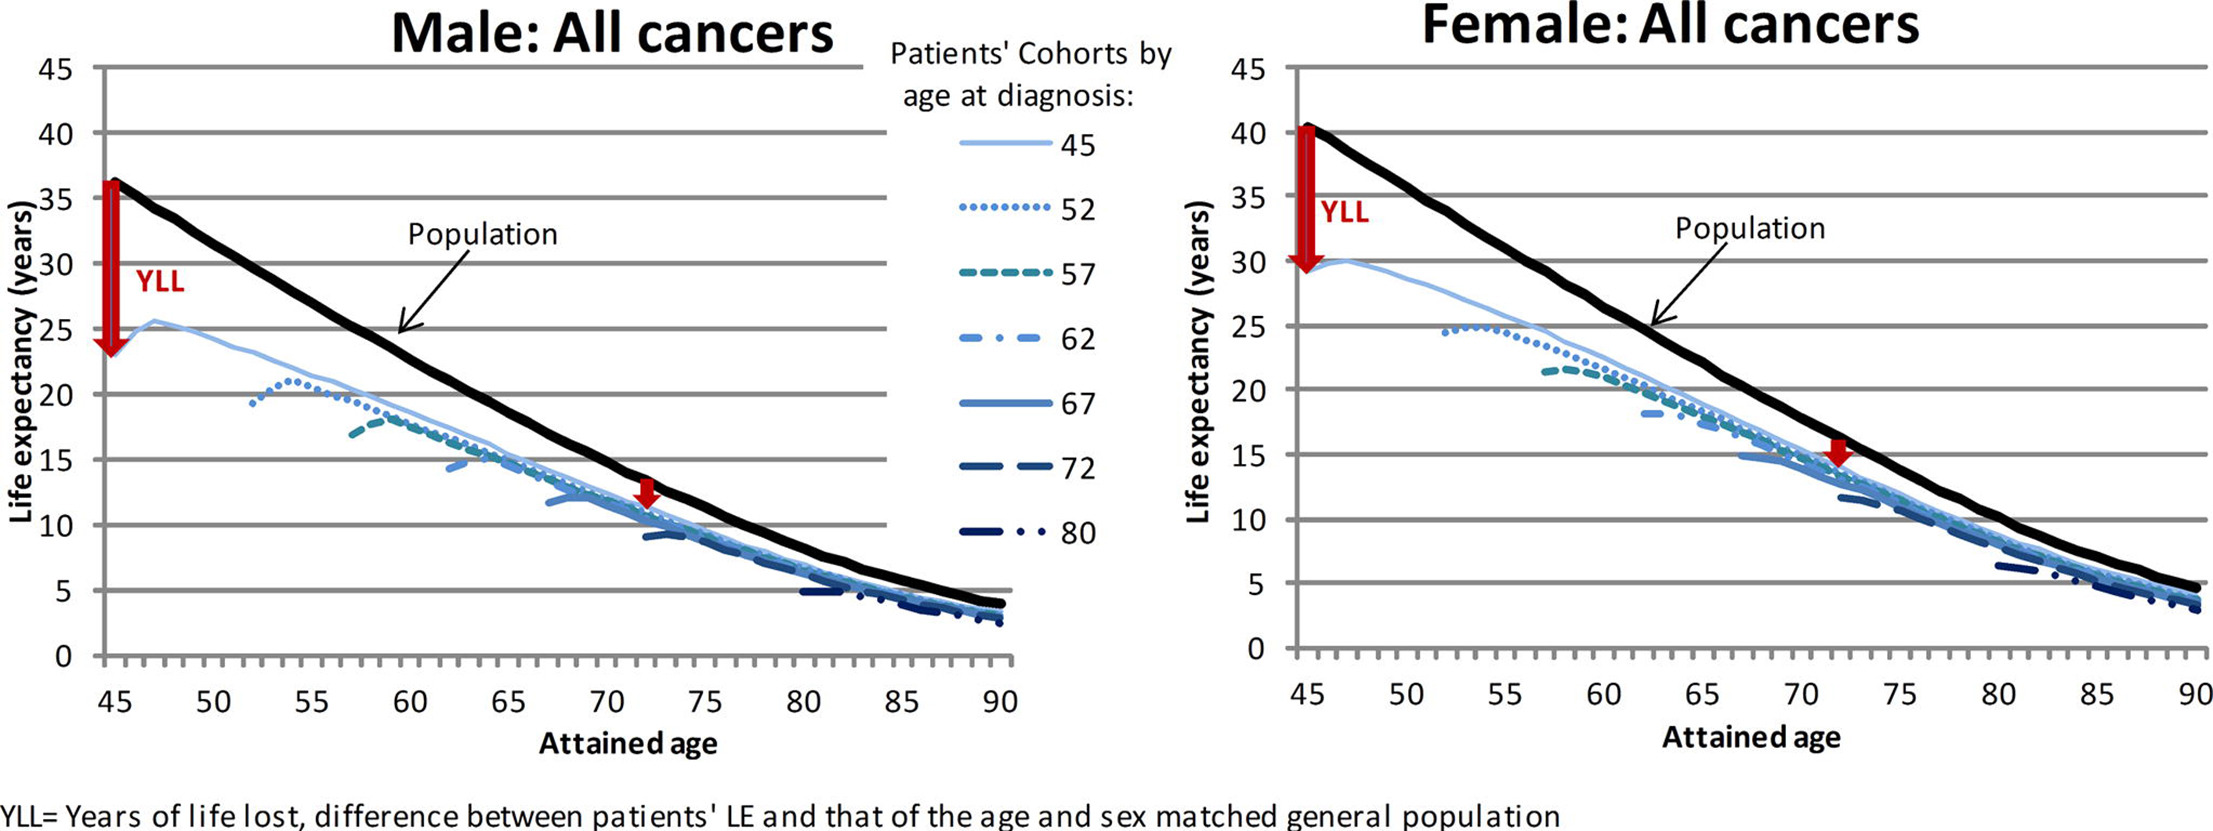
\includegraphics[width=\textwidth]{all_cancers_LE} \\
    \cite{botta2019changes}
    \newline
    \newline
    \pause
    Conclusion: Cancer causes the underlying \\ 'aging clock' to speed up
\end{frame}

\begin{frame}[c]{Life Expectancy with Diabetes}
    \large
    Life Expectancy is at least 10 years lower with Diabetes Type 1
    \cite{livingstone2015estimated} and at least 5 years lower with Diabetes Type
    2 \cite{untitled1:online}.
    \newline
    \newline
    \pause
    Conclusion: Diabetes causes the underlying \\ 'aging clock' to speed up
\end{frame}


\begin{frame}[c]{Life Expectancy under Physiological Stress}
    \large
    \begin{aquote}{John S Wentworth \cite{Homeosta76:online}}
    There's a qualitative general pattern that various kinds of physiological
        stress - exposure to radiation or harsh chemicals (including smoking),
        chronic infection, malnutrition, sleep deprivation, etc - tend to
        accelerate aging.
    \end{aquote}
\end{frame}


\subsection{Diseases of Aging}

\begin{frame}[c]{Similarities of Diseases of Aging}
    \large
    \cite{CorePath13:online}
    At the cellular level:
    \begin{itemize}[<+(1)->]
        \item Decrease in cell count
        \item Increase in damaged proteins/DNA/fats
        \item Inflammation
    \end{itemize}
    \pause

    Roughly this pattern for:
    \begin{multicols}{2}
    \begin{itemize}[<+(1)->]
        \item Alzheimers
        \item Arthritis
        \item Atherosclerosis
        \item Muscle loss
        \item Osteoporosis
        \item Many more
    \end{itemize}
    \end{multicols}
\end{frame}

\begin{frame}[c]{Existence proof for common pathways}
    \large
    \begin{aquote}{John S Wentworth}
        someone who has one severe illness early is likely to have others
    \end{aquote}

    \pause
    Most severe illnesses cause the 'aging clock' to speed up. Most diseases of
    aging have similar characteristics. This is direct evidence that there are
    {\em few underlying root causes} for aging.
\end{frame}


\subsection{Core Mechanisms}

\begin{frame}[c]{Overview of Core Mechanisms}
    \large
    \begin{itemize}[<+(1)->]
        \item DNA Damage
        \item Loss of Epigenetic Information
        \item Mitochondria low-energy state
        \item Telomere attrition
        \item Unsuppressed Transposons
    \end{itemize}
\end{frame}

\begin{frame}[c]{DNA Damage}
    turnaround a few days at most, does not accumulate - but, increase causes aging, just isn't root cause
\end{frame}

\begin{frame}[c]{Epigenetic Information Loss}
    most have turnaround of a few weeks, very unlikely to be actual cause (?) \\
    degrades over time with devastating effects, but unlikely to be root cause \\
    seems fine in gonades \\
\end{frame}


\begin{frame}[c]{Mitochondria}
    Produce energy, explain fail-state and ROS
\end{frame}

\begin{frame}[c]{Telomere attrition}

\end{frame}

\begin{frame}[c]{Transposons}
    cause DNA damage, though rather additionally, as species without transposons also age \\
    about 50\% of human dna are 'dead' (broken) transposons, about 100 (of 11 major families) are still active \\
    they are suppressed most of the time, but 'let loose' a bit on other pressing matters (e.g. repairing dna damage)
\end{frame}



\subsection{Assumed Root Causes}

\begin{frame}[c]{Problem: Many Theories}
    \large
    \begin{itemize}[<+(1)->]
        \item Everything is interlinked
        \item Very hard to distinguish cause and effect
        \item At least one Theory for every Hallmark
        \item Every prestigious lab has its own Theory
        \item A lot of speculation on all sides
        \item Unclear if we can already see the full picture
    \end{itemize}
\end{frame}


\addtocounter{framenumber}{1}
\begin{frame}[standout]
    Disclaimer: Purely Speculation including many Unknowns
\end{frame}

\begin{frame}[c]{Mitochondrial dysfunction}
    \large
    Turns out, mitochondrial dysfunction accounts for telomere-dependent senescence \cite{passos2007mitochondrial}.
\end{frame}


\begin{frame}[c]
    \large
    Assumed root causes: free radicals and transposon damage \\
    Maybe not in too much detail? Could fill 30min itself \cite{CorePath13:online} \\
    \pause

    p21 and reactive oxygen feedback for senescence \cite{passos2010feedback}
\end{frame}



\subsection{Open Questions}

\begin{frame}[c]{Questions Unanswered}
    \begin{itemize}[<+(1)->]
        \item Where are the ROS produced? Mitochondria are the top candidate - there’s a known mechanism for ROS production by mitochondria, as well as experimental evidence that mitochondrion-targeted antioxidants specifically reduce ROS-induced damage.
        \item How do the ROS and/or damaged molecules move between compartments, e.g. nucleus/cytoplasm/extracellular? I have seen very little on this, and consider it a major blindspot. I’m not sure if it’s a blindspot for the field or if I just haven’t found the right cluster of papers.
        \item Are the quantitative changes in DNA/protein/fat damage compatible with a single underlying cause? Do they match plausible estimates of ROS from dysfunctional mitochondria? Again, I haven’t seen Fermi estimates here, but I’d like to.
        \item Why is the immune system degradation related? It does degrade similarly over time, does it 'age' as well? This implies at least a second independent pathway and approach
    \end{itemize}
\end{frame}
